\section{System Framework}
\subsection{Development System Specification}
Processor : 1.3 GHz Intel Core i5\\*
Memory : 8 GB 1600 MHz DDR3\\*
Graphics : Intel HD Graphics 5000\\*
Software : OS X Mavericks - 10.9.4

\subsection{Data Collection Unit Technical Specification}
IDE : Eclipse Version 4.3.1 \\*
Langauge : Java \\*
Libraries :
\begin{itemize}
\item NorthContepts Datapipeline\footnote{http://northconcepts.com/data-pipeline/} : The Tweet data received from the Twitter API appears in JSON format. We would need to convert this to a CSV type file for our data analysis. After considering many other libraries, many of which require you to first convert JSON to Java Beans and then convert the Java Bean to CSV,  we decided to use Datapipeline by Nothconcepts for its integrated functionality. There were a couple of minor problems with this Library, but in general it worked well for our needs. 
\item Apache HttpComponents\footnote{http://hc.apache.org/} : This library is responsible for creating and maintaining a toolset of low level Java components focused on HTTP and associated protocols. We used this to build a custom client HTTP service for our `GET' requests from Twitter. 
\item Twitter API\footnote{https://dev.twitter.com/} : This is a REST API and is used to interact with the backend of Twitters' database. More information on retrieving Twitter feeds are given in Chapter 4. 
\end{itemize}

\subsection{Machine Learning Model Technical Specification}
IDE : Xcode Version 5.1.1 \\*
Language : Python \\*
Libraries :
\begin{itemize}
\item Pandas\footnote{http://pandas.pydata.org/} : Pandas is a very powerful data analysis toolkit for python. It provides fast, flexible and expressive data structures which makes working with relational or labelled data intuitive. Below are listed some of the reasons for me choosing Pandas :
\begin{itemize}
\item Python was the preferred programming language for the Machine Learning aspect of this project, however it is not very good at data analysis and modelling. The Pandas library fills this gap, hence we would not have to switch to another programming language for data analysis and/or modelling. 
\item It is easy to learn and use hence gave me more time to focus on the research.
\item Fast tabular data input/output : Very useful to load large data into python especially if the dataset is large.
\item Time series operation : We have a column that contains strings of the time stamps of the creation date of the tweets and you can use Pandas' timestamp format and set it as the index of the DataFrame. This could be useful if we want to represent the data as a collection of TimeSeries for some operation. 
\item Missing data handling : The results received from twitter had many missing data or no information available for particular features. Pandas handles missing data quite well, such as dropping rows, fill them with some value, or fill them with a computed value. This is not to say that other Libraries do not do the same, but just that Pandas handles this quite well. 
\item Group by, Merge and Join Operations : Pandas also gives you a way to do SQL type GroupBy , Merge and Join Operations. This could be useful to view the dataset in a different light. 
\item Data alignment : To create the union of two data frames or separating them. In my dataset we have tweets from different user accounts which we might at some point want to separate and analyse as well. One option would be to do this in Java, which is how we retrieved the data from twitter, however using Pandas it is faster and easier. 
\end{itemize}
\item Numpy\footnote{http://www.numpy.org/}  : Numpy adds support to large matrices and n-dimensional arrays and contains a huge library of mathematical functions which can be used on these arrays. 
\item MatplotLib\footnote{http://matplotlib.org/}  : This is a plotting package for python which was used to plot our data and other necessary plots. 
\item Re\footnote{https://docs.python.org/2/library/re.html}  : This module gives us regular expression matching functions, and is very similar to that in Perl. This was used in our program to identify patterns in the text of the tweet as well as user names etc. 
\item Sklearn\footnote{http://scikit-learn.org/}  : This was the library used for the Machine learning modules. 
\item Patsy\footnote{https://pypi.python.org/pypi/patsy/}  : Patsy is used to describe statistical models. We have used patsy to create our matrices. 
\end{itemize}

\section{Confusion Matrix}
\begin{figure}[!h]
 \centering
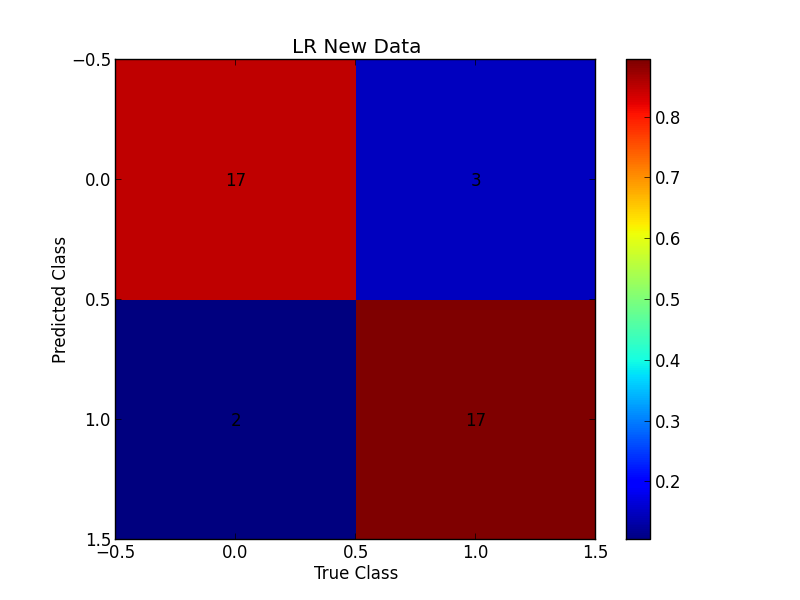
\includegraphics[width=10cm]{LRCMNewData}
  \caption[LR Confusion Matrix New Data]
   {LR Confusion Matrix New Data}
\end{figure}\leavevmode 

\begin{figure}[!h]
 \centering
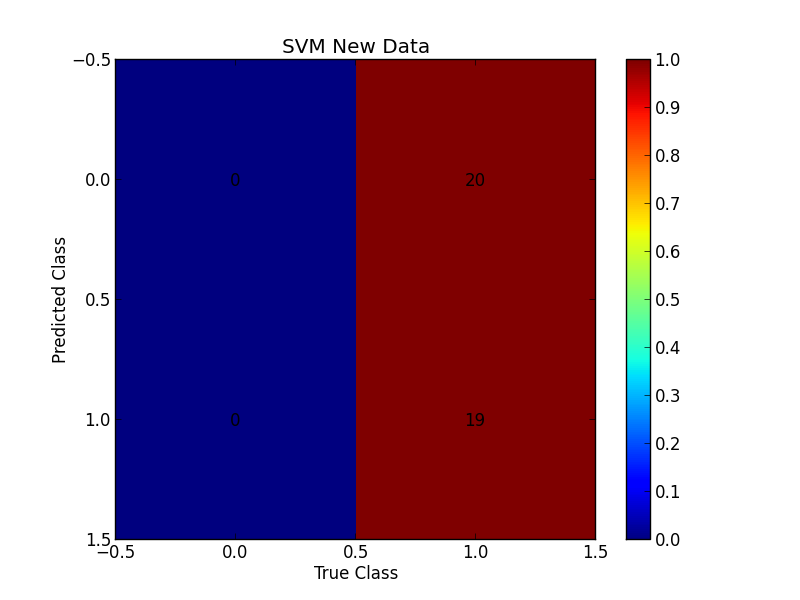
\includegraphics[width=10cm]{SVMCMNewData}
  \caption[SVM Confusion Matrix New Data]
   {SVM Confusion Matrix New Data}
\end{figure}\leavevmode 

\begin{figure}[!h]
 \centering
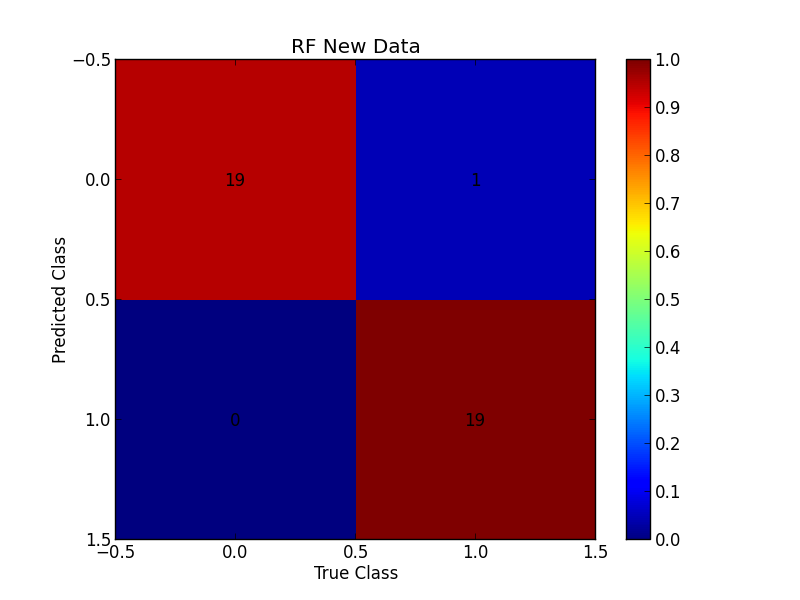
\includegraphics[width=10cm]{RFCMNewData}
  \caption[RF Confusion Matrix New Data]
   {RF Confusion Matrix New Data}
\end{figure}\leavevmode 

\begin{figure}[!h]
 \centering
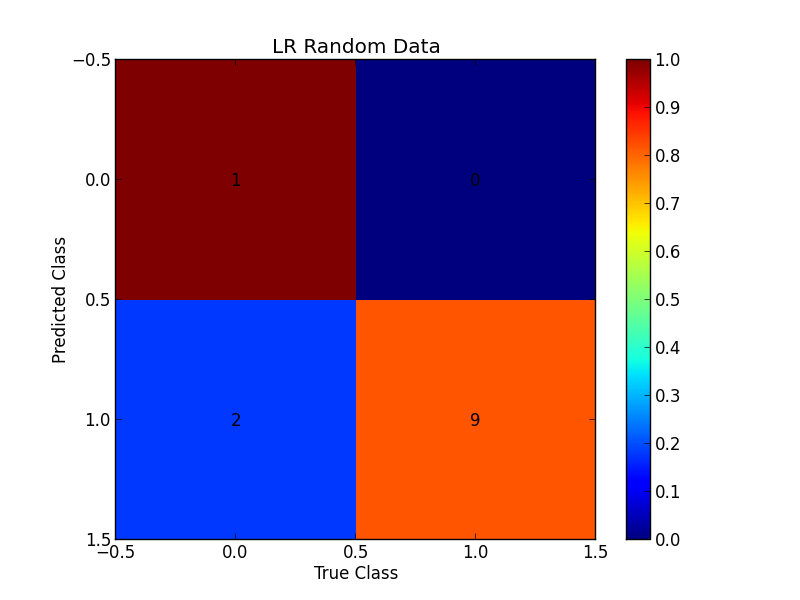
\includegraphics[width=10cm]{LRCMRandomData}
  \caption[LR Confusion Matrix Random Data]
   {LR Confusion Matrix Random Data}
\end{figure}\leavevmode 

\begin{figure}[!h]
 \centering
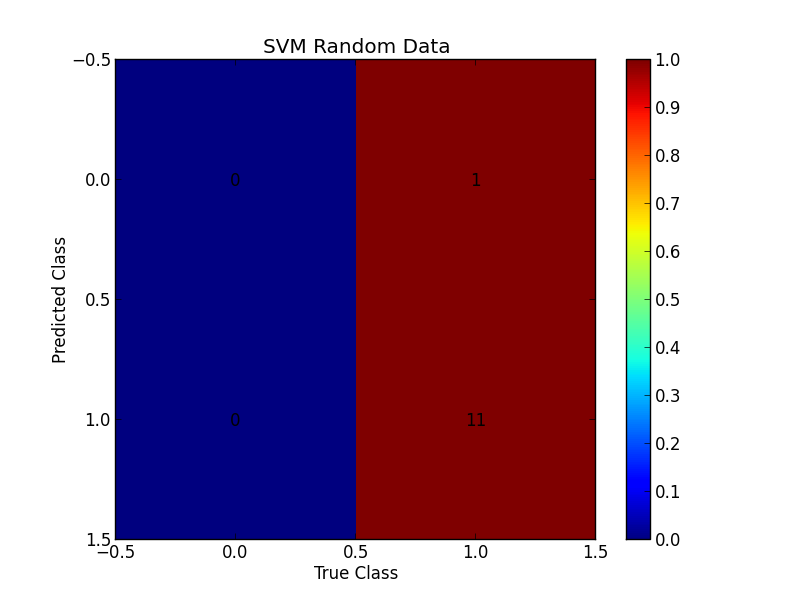
\includegraphics[width=10cm]{SVMCMRandomData}
  \caption[SVM Confusion Matrix Random Data]
   {SVM Confusion Matrix Random Data}
\end{figure}\leavevmode 

\begin{figure}[!h]
 \centering
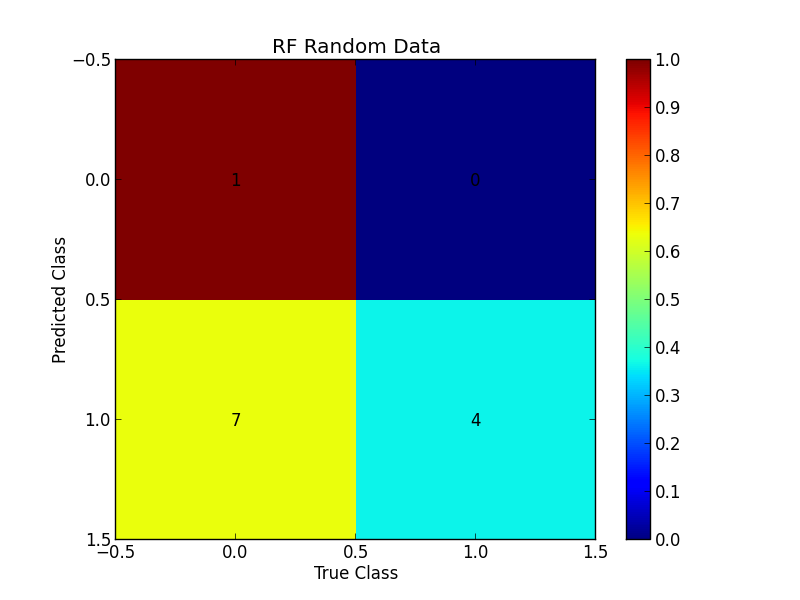
\includegraphics[width=10cm]{RFCMRandomData}
  \caption[RF Confusion Matrix Random Data]
   {RF Confusion Matrix Random Data}
\end{figure}\leavevmode 